% Evolvable systems on reconfigurable architecture via self-aware adaptive applications. ++
\cite{evolvable} proposes an evolvable system exploiting self-adaptive techniques by running a customized version of GNU/Linux and a set of adaptive applications on top of a heterogeneous system featuring a multi-core Intel Core i7 processor and a reconfigurable device, a Xilinx Virtex 5. The underlying hardware architecture is made up of static area, containing the general purpose processor and a dynamic area which contains the FPGA. 

The customized operating system provides common functionalities through standard libraries and is able to choose at runtime the best implementations for the required functionalities thanks to a set of self-adaptive libraries. Depending on the linked library, applications can either be standard or self-adaptive. They come up with an agile decisioning framework driven by a heuristic policy based on an empiric model. This policy should avoid osciliating behavior as to not interfere with the Heartbeats application that is used as a monitoring technique. This 3 tier system can be seen in figure \ref{fig:tier}.
%
%
% -- plaatje 3 tier architecture ---------------------------
\begin{figure}[htb]%
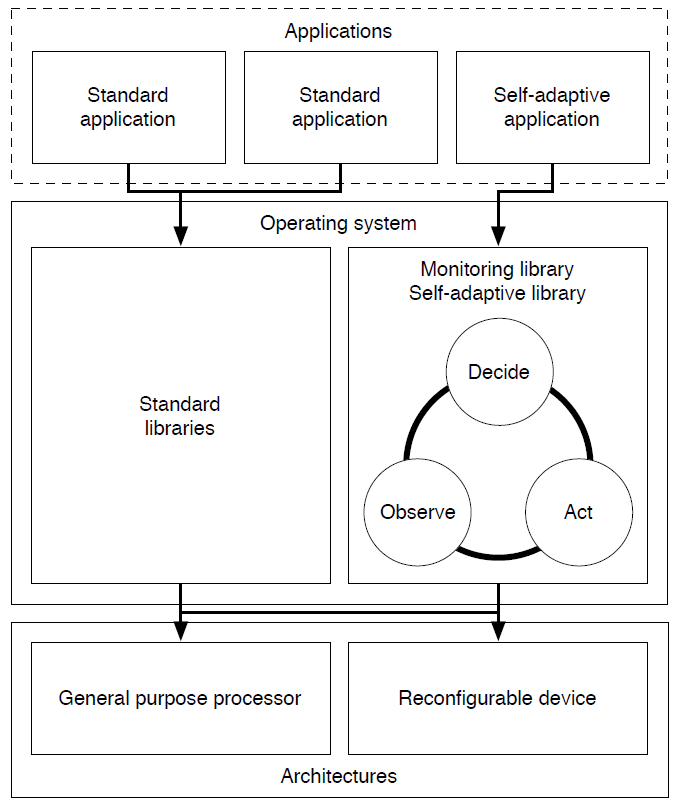
\includegraphics[width=\columnwidth]{Pictures/3tier.png}%
\caption{Overview of the evolvable system as seen in \cite{evolvable}, providing self-adaptive libraries}%
\label{fig:tier}%
\end{figure}

The online reconfiguration mechanism proposed in \cite{evolvable} is inspired by the modern object oriented operating system called K42, developed by IBM. For the hot-swap mechanism they define a \emph{switchable unit} with a clearly defined interface, \emph{state quiescence} for each access is mutually exclusive and states are maintained per-thread and the \emph{state translation} problem is solved by converting user data back-and-forth from a canonical data structure to the specific data structure used by the active implementation library. They conclude by presenting their implementation of evolvable self-adaptive methods on a heterogeneous architecture as observe-decide-act loops, capable of meeting the given performance goals. 

